\chapter{Lensing convergence and neutrino mass in galaxy surveys}
\label{chapter-mnu}

\section{Introduction}
\label{chapter-mnu:introduction}

Measurements of the Cosmic Microwave Background (CMB) anisotropies over the past three decades represent a remarkable achievement in cosmology \cite{Smoot:1992td,Bennett:2003bz,Ade:2013sjv}. Constant increases in both amount and quality of data not only have allowed more rigorous tests of cosmological models, but also have required the improvement of both the tools and methods we use for the analysis of those data sets. This progress has turned out in a phenomenological model of the universe which fits reasonably well most of the available observations \cite{Ade:2015xua}.    

Although the $\Lambda CDM$ model is relatively successful at explaining the current observations, most of the underlying physics in the model remains unknown (e.g., dark energy, dark matter). In particular, the unknown Cold Dark Matter (CDM) constitutes about $30\%$ of the energy content in the universe. Searches for dark matter particles have come out with no conclusive results, leaving neutrinos as the only known dark matter candidate. Neutrino experiments have shown that neutrinos are massive particles, but have been unable to provide an absolute scale for their masses \cite{Lesgourgues:2006nd,Lesgourgues:2012uu}. 

Since massive neutrinos change the background evolution of the universe, CMB measurements can be utilised to constraint their masses. When the neutrino mass is small ($\approx 0.1 \, \mathit{eV}$) neutrinos have a modest signature on the CMB angular power spectrum and those constraints can provide only an upper limit for the neutrino mass. Degeneracies with other parameters in the cosmological model (e.g., the equation of state of dark energy $w$ or the Hubble parameter $H_0$) help to further degrade constraints on the neutrino mass from CMB data.  
   
By mapping the distribution of matter in the universe one can also test cosmological models. Galaxy surveys, probing the low red-shift universe, allow to break parameter degeneracies hence improving the constraints on the neutrino masses  \cite{Hu:1997mj}. Massive neutrinos would suppress the clustering of galaxies at small scales thus damping the matter power spectrum $P(k)$ on those scales. It is expected that future galaxy surveys will be able to measure this suppression and therefore determine the  absolute mass of the neutrinos.  
  
Future galaxy surveys will probe distance scales comparable to the Hubble horizon (a few tens of $\mathrm{Gpc^3/h^3}$) thus allowing more rigorous analysis. Non-linearities and relativistic effects such as red-shift space distortions and lensing convergence should then be consistently included in galaxy clustering analyses if the constraining power of the survey is not to be wasted. This chapter aims at showing the importance of the inclusion of lensing convergence in galaxy clustering analyses. In particular, we show that if future analyses neglected the lensing convergence, measurements of the neutrino masses would be severely biased thus throwing away valuable information and leading to misleading conclusions about the cosmological model. 

The plan of the chapter is as follows. In the next Section we recall how galaxy number counts are modelled. Our methodology is explained in Section \ref{chapter-mnu:methodology}. Then in Section \ref{chapter-mnu:results} we show and discuss our results. Finally, we give our conclusions in Section \ref{chapter-mnu:conclusions}.

\section{Galaxy number counts angular power spectrum}
\label{chapter-mnu:modelling}

Although galaxy red-shift surveys measure red-shift $z$ and direction $\mathbf{n}$ of sources in the sky, analyses of galaxy clustering data are commonly done by using the matter power spectrum $P(k,z)$ \cite{Feldman:1993ky} which is not an observable. An alternative approach uses the angular matter power spectrum $C_\ell(z,z')$ which is an observable. It has been shown in \cite{DiDio:2013sea} that for galaxy catalogues with photometric red-shifts, an analysis of the $C_\ell(z,z')$ spectra can perform significantly better than one using $P(k,z)$. This is due to both an optimal use of red-shift information and the not averaging over directions in the $C_\ell(z,z')$ approach. It is therefore more suitable to work with the angular matter power spectrum and we have chosen to do so in this project.  

Galaxy number counts for a survey with limiting magnitude $m_{\mathrm{lim}}$ is given by 
\begin{equation}
\label{Eq:galaxy-number-counts}
n(z,\mathbf{n};\,m_{\mathrm{lim}}) = \bar{n}(z) \left[ 1 + \Delta(z,\mathbf{n};m_{\mathrm{lim}}) \right],
\end{equation}  
where $\bar{n}(z)$ is the mean galaxy density per red-shift and per steradian at red-shift $z$, and 
\begin{eqnarray}
\label{Eq:galaxy-number-counts-perturbation}
\Delta(z,\mathbf{n};m_{\mathrm{lim}}) &=&  b(z) D + \frac{1}{\H}\left[ \dot{\Phi} + \partial_r^2 V \right] + (2 - 5 s) \left[ \int_0^r \frac{d\tilde{r}}{r}(\Phi + \Psi) - \kappa \right] \nonumber \\
&+&  (f_{\mathrm{evo}} - 3)\H V + (5s-2)\Phi + \Psi 
+ \left( \frac{\dot{\H}}{\H^2} + \frac{2 - 5s}{r\H} + 5s - f_{\mathrm{evo}} \right) \nonumber \\
&\times & \left( \Psi + \partial_rV + \int_0^r d\tilde{r}(\dot{\Phi} + \dot{\Psi}) \right) 
\end{eqnarray}
is the perturbation in the number density of sources which emerges due to both red-shift density perturbations and volume distortions \cite{Bonvin:2011bg,Challinor:2011bk,Yoo:2012se}. In Eq. \eqref{Eq:galaxy-number-counts-perturbation}, $b(z)$ takes into account that galaxies are biased tracers of the underlying dark matter distribution, $D$ is the density fluctuation in comoving gauge, $\H \equiv aH$ is the conformal Hubble parameter, $\Phi$ and $\Psi$ are the Bardeen potentials \cite{Bardeen:1980kt}, $V$ is the velocity potential for peculiar velocities in the longitudinal gauge, $v_i=-\partial_i V$, $s$ is the magnification bias , $\kappa$ is the convergence, $r$ is the comoving distance, $f_{\mathrm{evo}}$ is the evolution bias, and a dot denotes derivative w.r.t. conformal time. Both the evolution bias and the magnification bias functions are defined below when giving the survey specifications. 

Similarly to what is done in CMB analysis with temperature fluctuations, it is useful to expand the perturbation in the number density of galaxies in spherical harmonics $Y_{\ell\,m}(\mathbf{n})$. Whereas for the CMB case one expands the temperature fluctuations field $\Delta T(\mathbf{n})$ at a single red-shift ($z\sim 1000$), when analysing galaxy catalogues we have data for a range of red-shifts and therefore the expansion takes into account this red-shift dependence
\begin{equation}
\label{Eq:galaxy-number-counts-perturbation-expansion}
\Delta(z,\mathbf{n}) = \sum_{\ell,m} a_{\ell m}(z) Y_{\ell m}(\mathbf{n}), 
\end{equation}   
where we have omitted the limiting magnitude. Assuming statistical isotropy, it is possible to define the angular matter power spectrum through the expansion \eqref{Eq:galaxy-number-counts-perturbation-expansion} as
\begin{equation}
\label{Eq:definition-angular-matter-power-spectrum}
\langle a_{\ell m}(z) a^*_{\ell m}(z') \rangle \equiv \delta_{\ell \ell'} \delta_{m m'} C_\ell(z,z').
\end{equation} 

In practice, galaxy clustering data is commonly analysed by using tomographically binned samples of galaxies. The catalogue can be divided in different red-shift bins according to normalised window functions $W_{\Delta z_i}(z,z_i)$ of width $\Delta z_i$ and centred in red-shift $z_i$. One can then define correlations between red-shift bins $i$ and $j$ as
\begin{equation}
\label{Eq:binned-angular-matter-power-spectrum}
C_\ell^{ij} \equiv \int dz dz' W_{\Delta z_i}(z,z_i) W_{\Delta z_j}(z,z_j) C_\ell (z,z').
\end{equation} 
In this project we have used synthetic galaxy clustering data for a survey consistent with the Euclid photometric catalogue:
\begin{itemize}
\item the covered sky fraction $f_{\mathrm{sky}}=0.364$; 
\item we divide the catalogue into $N_{\mathrm{bin}}=5$ Gaussian red-shift bins (Gaussian window functions $W_{\Delta z_i}$) containing equal number of galaxies;
\item the galaxy red-shifts are assumed to range from $0.1$ to $2$;
\item the galaxy density $d=30\,\mathrm{arcmin^{-2}}$;
\item the number of galaxies per red-shift and per steradian 
\begin{equation}
\label{Eq:dNdzdOmega}
\dfrac{dN}{dzd\Omega} = 3.5\times 10^8 z^2 \exp \left[-\left( \frac{z}{z_0} \right)^{3/2} \right] \qquad z_0=0.637, 
\end{equation}
is shown in Figure \ref{fig:dNdz};
\item the number of galaxies per steradian within a given red-shift bin is 
\begin{equation}
\label{Eq:number-galaxies-per-bin}
\N = \frac{1}{N_{\mathrm{bin}}}\int dz \dfrac{dN}{dzd\Omega};
\end{equation}
\item as suggested by previous studies (see, for instance, \cite{Tegmark:2003uf}) we assume a scale-independent galaxy bias 
\begin{equation}
b(z) = b_0\sqrt{1+z};
\label{Eq:galaxy-bias}
\end{equation}
\item following \cite{Montanari:2015rga}, the magnification bias for an Euclid-like survey is modelled as 
\begin{equation}
s(z) = \sum_{k=0}^3 s_k z^k,
\label{Eq:magnification-bias}
\end{equation}
with $s_0 = 0.1194,\, s_1 = 0.2122,\, s_2 = -0.0671,\, s_3 = 0.1031$;
\item finally, the evolution bias 
\begin{equation}
f_{\mathrm{evo}}(z) \equiv \dfrac{\partial \ln \left( a^3 \dfrac{dN}{dzd\Omega}  \right)}{\partial \ln a},
\label{Eq:evolution-bias}
\end{equation}    
where $a$ is the scale factor and we assume that the survey observes all the galaxies in the windows. The galaxy bias and the magnification bias are shown in Figure \ref{fig:bs}.
\end{itemize}   

\begin{figure}[hbtp]
%\vspace{0.3cm}
\begin{center}
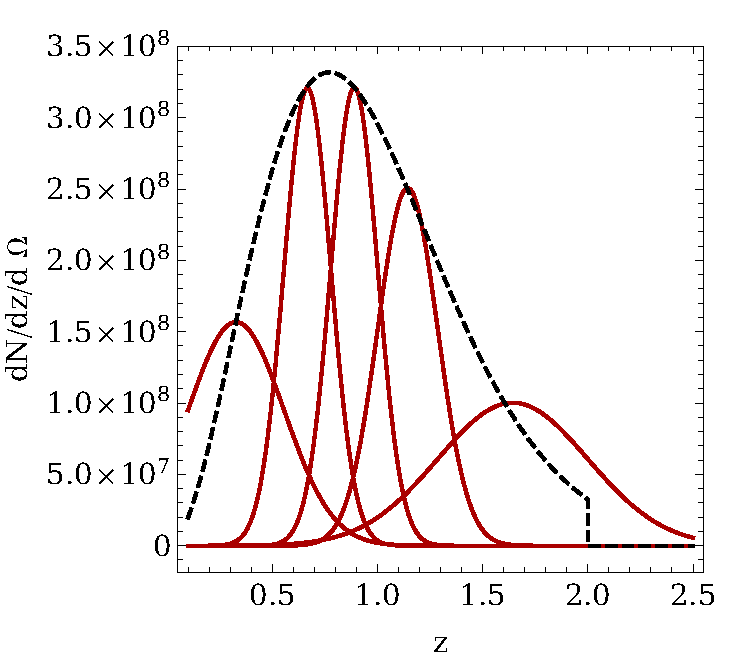
\includegraphics[width=\textwidth]{figures/chapter-mnu/euclid_5bin.pdf}
\end{center}
\caption{Euclid photometric galaxy density distribution (black line) with a division into 5 bins containing the same number of galaxies.
}
\label{fig:dNdz}
\end{figure}

%
\begin{figure}[hbtp]
\begin{center}
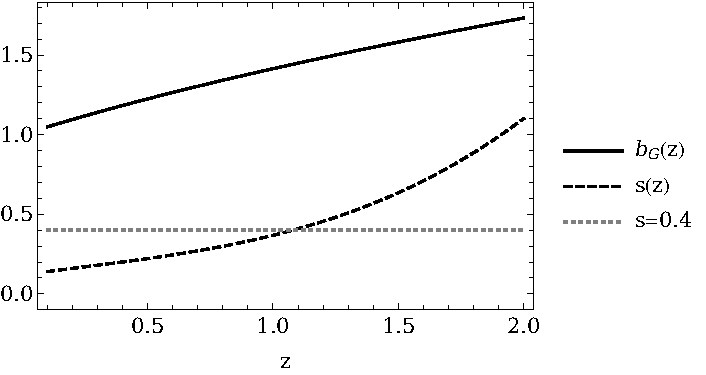
\includegraphics[width=\textwidth]{figures/chapter-mnu/bs.pdf}
\end{center}
\caption{Galaxy bias $b_G(z)$ and magnification bias $s(z)$ for Euclid. The
magnification bias is computed at the limiting magnitude $m_{\rm lim}=24.5$.
As a reference, we also plot the value $s=0.4$ at which the lensing contribution to number counts changes sign.
}
\label{fig:bs}
\end{figure}

Having the survey specifications we can compute angular matter power spectrum as in Eq. \eqref{Eq:binned-angular-matter-power-spectrum}. We have utilised the code CLASSgal \cite{DiDio:2013bqa} where galaxy number counts have been implemented including relativistic corrections in Eq. \eqref{Eq:galaxy-number-counts-perturbation}. 
%In Figure \ref{Fig:comparison-massive-massless-Cls} we compare galaxy number counts angular power spectrum for a model with massive neutrinos and a model where neutrinos are massless. 
In the next section we study the importance of including the effect of lensing convergence in galaxy clustering analyses when determining the neutrino mass. 

%\begin{figure}[hbtp]
%\begin{center}
%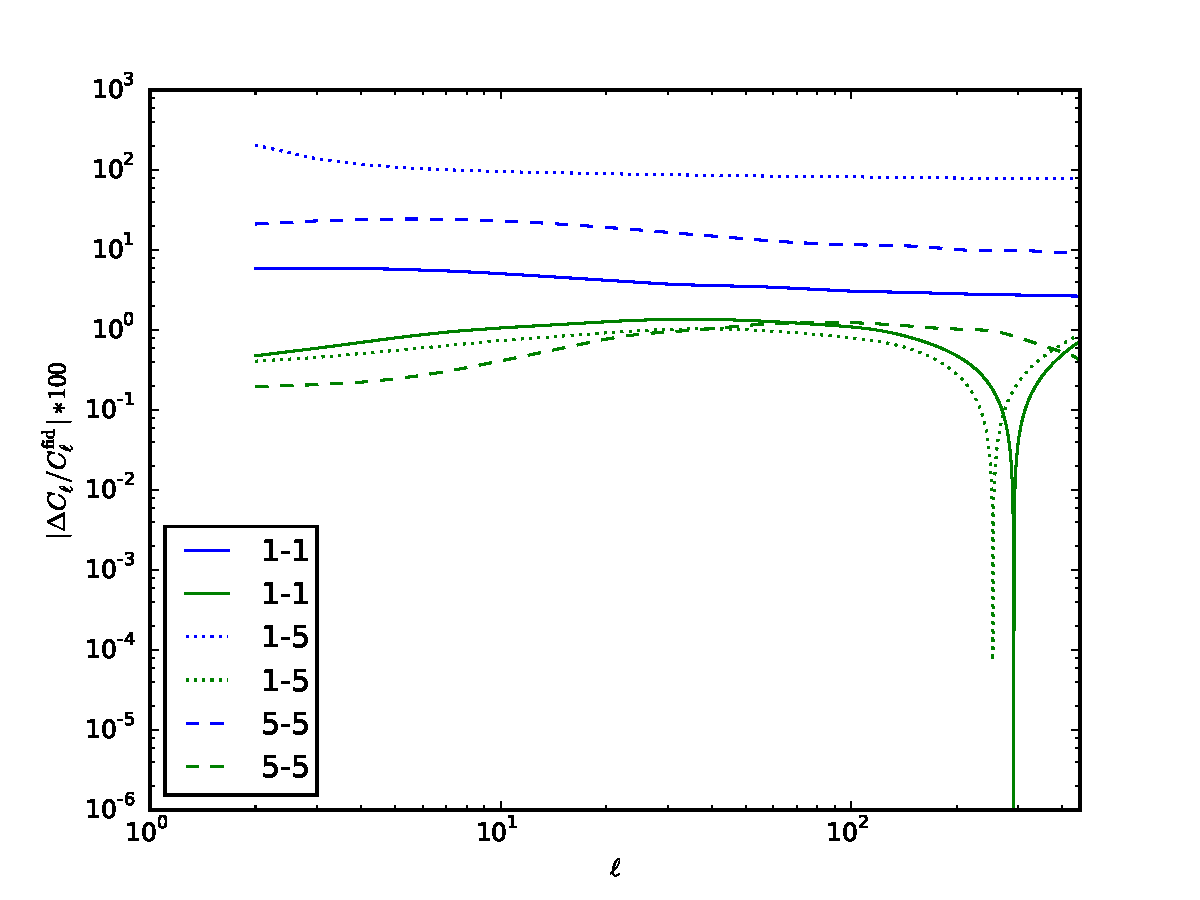
\includegraphics[width=\textwidth]{figures/chapter-mnu/correlation_comparison.pdf}
%\end{center}
%\caption{Percentage relative difference of correlations Blue illustrates the difference between models with and without lensing convergence. Green compares models with and without massive neutrinos. Comparison auto and cross-corelations for models with and without neutrino mass}
%\label{Fig:comparison-massive-massless-Cls}
%\end{figure}
 
\section{Methodology}
\label{chapter-mnu:methodology}

In order to show how important the inclusion of lensing convergence in galaxy clustering analyses is, we perform a Markov Chain Monte Carlo (MCMC) analysis \cite{Lewis:2002ah,Verde:2003ey,Tegmark:2003ud} both including and neglecting the lensing effect. Studies analysing the bias on cosmological parameters due to neglecting lensing convergence can be found in the literature, but they do Fisher matrix analyses and focus on either the primordial non-Gaussianity parameter (i.e., $\fNL$) \cite{Namikawa:2011yr} or dark energy parameters (e.g., $w,\, \Omega_\Lambda$) \cite{Duncan:2013haa}. Although in this project we stress on the neutrino mass, we also discuss other parameters in the concordance model.  

The MCMC technique is more suitable than a Fisher matrix method. Current Boltzmann codes such as CLASS \cite{Lesgourgues:2011re} or CAMB \cite{Lewis:1999bs} are accurate to $1\%$ (with nominal precision settings), but it is possible for random numerical errors to exceed this. Future surveys will provide more precise Large Scale Structure (LSS) measurements and therefore these effects might become problematic for approaches that rely on computation of derivatives as a function of parameters (e.g., Fisher matrix). Since our MCMC approach average over $\sim 10^5$ galaxy number counts spectra, it is much less sensitive to those numerical errors than the Fisher matrix approach. 

We assume a fiducial flat $\Lambda CDM$ model consistent with results from the Planck collaboration \cite{Ade:2015xua}, including massive neutrinos with a normal mass hierarchy (dominated by the heaviest neutrino mass eigenstate). The cosmological parameters of our fiducial model are the reduced baryon density parameter, $\omega_{\mathrm{b}} = 2.225\times 10^{-2}$, the cold dark matter density parameter, $\omega_{\mathrm{cdm}}=0.1198$, the scalar spectral index, $n_{\mathrm{s}}=0.9645$, the amplitude of curvature fluctuations, $\ln 10^{10} A_{\mathrm{s}}=3.094$, the Hubble constant, $H_0 = 67.27\, \mathrm{km\, s^{-1}\, Mpc^{-1}}$, and the sum of the neutrino masses, $\sum m_\nu = 0.06\, \mathrm{eV}$.  
     
To take into account a theoretical error on non-linear scales we use Halofit \cite{Smith:2002dz} to rescale all linear transfer functions. The rescaling for the matter power spectrum in models including massive neutrinos has been already implemented in CLASSgal. Transfer functions are rescaled by the square root of 
\begin{equation}
\alpha(k,z) = \frac{\ln [1 + k/k_{\mathrm{NL}(z)}]}{1 + \ln [1 + k/k_{\mathrm{NL}(z)}]}f_{\mathrm{th}},
\label{Eq:rescaling-factor-transfer-functions}
\end{equation}
where $k_{\mathrm{NL}}$ is the non-linear scale determined by the Halofit algorithm, and $f_{\mathrm{th}}$ is the error percentage on non-linear scales that we have chosen to be $f_{\mathrm{th}}=10\%$. The theoretical error power spectra $E_\ell^{ij}$ are then computed by taking the absolute value of the resulting $C_\ell^{ij}$. Because computing $E_\ell^{ij}$ with high accuracy is time-computing demanding, in this project we compute the error power spectra only for the fiducial model, that is, we ignore the parameter dependence on the theoretical error. In addition, since the  perturbation on the number density of galaxies is not a continuous field, it is usually assumed that galaxies form a Poisson sample of the density field \cite{Feldman:1993ky} and therefore there is a shot-noise contribution $\N^{-1}$ to the error budget in the angular power spectra.

Finally, the galaxy number counts are modelled as 
\begin{equation}
\label{Eq:GNC-modelled-angular-power-spectra}
C_\ell^{A,\,ij} = C_\ell^{ij} + E_\ell^{ij} + \N^{-1} \delta^{ij},
\end{equation}
where $A=\mathrm{obs},\,\mathrm{th}$ and $i,j = 1,...,N_{\mathrm{bin}}$ are red-shift bin indices. Here $C_\ell^{\mathrm{obs}}$ stands for spectra computed for our fiducial model which includes the effect of lensing convergence, and $C_\ell^{\mathrm{th}}$ stands for models which might or might not include lensing convergence. In the next Section we will study the impact of switching lensing convergence off in $C_\ell^{\mathrm{th}}$ when fitting this kind of models to our fiducial $C_\ell^{\mathrm{obs}}$.   
     
Following the cosmic shear implementation in \cite{Audren:2012vy} we have implemented a Gaussian likelihood for an Euclid-like survey. For given observed and theoretical power spectra in Eq. \eqref{Eq:GNC-modelled-angular-power-spectra}, let us define the determinants
\begin{eqnarray}
\label{Eq:determinants-Gaussian-likelihood}
d_\ell^{\mathrm{th}} & = & \det \left( C_\ell^{\mathrm{th},\,ij}\right),\\
d_\ell^{\mathrm{obs}} & = & \det \left( C_\ell^{\mathrm{obs},\,ij}\right). 
\end{eqnarray}
Additionally, one can define a mixed determinant $d_\ell^{\mathrm{mix}}$ formed from $d_\ell^{\mathrm{th}}$: one takes each term in $d_\ell^{\mathrm{th}}$ and replaces one at a time $C_\ell^{\mathrm{th},\,ij}$ by the corresponding $C_\ell^{\mathrm{obs},\,ij}$. If we worked with $2$ red-shift bins, the mixed determinant would read
\begin{equation}
\label{Eq:example-mixed-determinant}
d_\ell^{\mathrm{mix}} = C_\ell^{\mathrm{obs},\,11}C_\ell^{\mathrm{th},\,22} + C_\ell^{\mathrm{th},\,11}C_\ell^{\mathrm{obs},\,22} - 2 C_\ell^{\mathrm{th},\,12}C_\ell^{\mathrm{obs},\,12}.
\end{equation}
                        
It is known that in an ideal full-sky experiment, the different multipoles in an spherical harmonics expansion of a given function are uncorrelated. Then in this simple case one can write the Gaussian likelihood
\begin{equation}
\label{Eq:GNC-Gaussian-likelihood}
\L = \widetilde{\N} \Pi_\ell \left\lbrace \frac{1}{(d_\ell^{\mathrm{th}})^{\frac{2\ell+1}{2}}} \exp \left[ -\frac{(2\ell+1)}{2} \frac{d_\ell^{\mathrm{mix}}}{d_\ell^{\mathrm{th}}}\right] \right\rbrace,                         
\end{equation}
where $\widetilde{\N}$ is a normalisation constant. The effective chi square is defined as
\begin{equation}
\label{Eq:GNC-effective-chi2}
\chi^2_\eff \equiv -2 \ln \L = -2 \ln \widetilde{\N} + \sum_\ell (2\ell+1)\left( \ln d_\ell^{\mathrm{th}} + \frac{d_\ell^{\mathrm{mix}}}{d_\ell^{\mathrm{th}}} \right), 
\end{equation}
which is minimal for $d_\ell^{\mathrm{mix}}= N_{\mathrm{bin}} d_\ell^{\mathrm{th}} = N_{\mathrm{bin}} d_\ell^{\mathrm{obs}}$. Having into account the partial sky coverage these definitions lead to a $\chi^2$ relative to the fiducial model given by                     
\begin{equation}
\label{Eq:relative-chi2}
\Delta \chi^2 = \sum_{\ell=2}^{\ell_{\mathrm{max}}} (2\ell+1) f_\fsky \left( \ln \frac{d_\ell^{\mathrm{th}} }{d_\ell^{\mathrm{obs}}} + \frac{d_\ell^{\mathrm{mix}}}{d_\ell^{\mathrm{th}}} - N_{\mathrm{bin}} \right),
\end{equation}                           
where to be conservative in the treatment of non-linear effects we use $\ell_{\mathrm{max}}=400$. In order to optimise the computation of the angular power spectra $C_\ell^{\mathrm{A},\,ij}$ we use the Limber approximation and adjust the precision parameters in CLASSgal to have $\Delta \chi^2 \lesssim 0.2$ for $C_\ell^{\mathrm{th}}$ including lensing evaluated at the fiducial model. These adjustments are necessary to make feasible our MCMC approach and mean that our computations are accurate up to $\Delta \chi^2 \lesssim 0.2$.                              
                                                                      
\section{Results}
\label{chapter-mnu:results}

Utilising the approach explained in Section \ref{chapter-mnu:methodology}, we have performed the three following MCMC  analyses:

\begin{enumerate}
\item $C_\ell^{\mathrm{th}}$ including lensing convergence.
\item $C_\ell^{\mathrm{th}}$ neglecting lensing convergence.
\item $C_\ell^{\mathrm{th}}$ neglecting lensing convergence, but including only auto-correlations.
\end{enumerate}

We have done these analyses in two ways. First, we assume no previous information and use wide, flat prior distributions for the cosmological parameters. Second, we consider a more realistic scenario where information from a full-sky CMB experiment is provided. In this case we assume a Gaussian prior distribution for the pertinent cosmological parameters; we compute the covariance matrix for a model with varying neutrino mass from information provided by the Planck collaboration. In addition to these two analyses, we do a Fisher matrix analysis no using priors and compare results with the corresponding MCMC analysis. We close this section by estimating the significance of lensing detection with an Euclid-like survey.

\subsection{MCMC with wide, flat priors}

The Figure \ref{fig:mcmc} shows two- and 1-D posteriors for the three mentioned analyses using wide, flat priors on the cosmological parameters. The corresponding constraints are shown in Table \ref{Table:1}. Red contours indicate results for the analysis that consistently includes lensing convergence in the theoretical model fitting the mock data. The analysis neglecting lensing convergence, but including only red-shift bin auto-correlations (i.e.\ $C_\ell(z,z)$), is depicted in gray. Blue contours show the analysis neglecting lensing, but including all possible red-shift bin correlations (i.e.\ $C_\ell(z,z')$).      

% \begin{table}[!tbhp]
\begin{table}[!t]
  \centering
  \begin{tabular}{@{}cccccc}
    \hline
    \multicolumn{6}{c}{i) Consistently including lensing: $\Delta \chi^2 = 0$} \\
    \hline
    Parameter & Mean & best fit & $\sigma$ &\hspace{-0.52cm} shift: mean & best-fit \\
    \hline
    $\omega_b$ & $0.02979$ & $0.02285 $ &$0.00624 $ &  \quad$1.2\sigma$ & $ 0.1\sigma$ \\
    $\omega_{cdm}$ & $0.1455 $ & $0.1219 $ & \quad$0.0200 $ &  \quad$1.3\sigma$ & $0.1\sigma$ \\
    $n_s$      & $0.9476 $ & $0.9642 $ & $0.0387 $ &  \quad$0.4\sigma$ & $ <0.1\sigma$ \\
    $\ln10^{10}A_s$ & $3.047 $ & $3.097$ & $0.065 $ &  \quad$0.7\sigma$ & $ <0.1\sigma$ \\
    $H_0\left[\frac{\text{km}}{\text{s}\cdot\text{Mpc}}\right]$      & $73.84$ & $67.84$ & $5.48$ &  \quad$1.2\sigma$ & $ 0.1\sigma$ \\
    $m_{\nu}$\,[eV]  & $0.29$ & $0.09$ & $0.19$ & \quad $ 1.2\sigma$ & $ 0.2\sigma$ \\
    $b_0$ & $1.018$ & $1.000$ & $0.031$ & \quad$0.6\sigma$ & $<0.1\sigma$ \\
  \end{tabular}
  \begin{tabular}{@{}cccccc}
    \hline
    \multicolumn{6}{c}{ii) Neglecting lensing: $\Delta \chi^2 = 2064$} \\
    \hline
    Parameter & Mean & best fit & $\sigma$ & \hspace{-0.52cm} shift: mean & best-fit \\
    \hline
    $\omega_b$ & $0.02494$ & $0.02120 $ & $0.00556 $ &  \quad$0.5\sigma$ & $0.1\sigma$ \\
    $\omega_{cdm}$ & $0.1532$ & $0.1435$ & $0.0208$ &  \quad$1.6\sigma$ & $1.1\sigma$ \\
    $n_s$      & $0.8702$ & $0.8837$ & $0.0446$ &  \quad$2.1\sigma$ & $1.8\sigma$ \\
    $\ln10^{10}A_s$ & $ 2.867 $ & $2.965 $ & $ 0.394 $ &  \quad$0.6\sigma$ & $0.3\sigma$ \\
    $H_0\left[\frac{\text{km}}{\text{s}\cdot\text{Mpc}}\right]$      & $68.73$ & $66.76$ & $5.14$ &  \quad$0.3\sigma$ & $0.1\sigma$ \\
    $m_{\nu}$\,[eV]  & $0.43$ & $0.41$ & $0.16$ &  \quad$2.3\sigma$ & $2.2\sigma$ \\
    $b_0$ & $1.293$ & $1.200$ & $0.271$ & \quad$1.1\sigma$ & $0.7\sigma$\\
  \end{tabular}
  \begin{tabular}{@{}cccccc}
    \hline
    \multicolumn{6}{c}{\parbox[t]{4.4cm}{iii) Neglecting lensing: \\ \hspace*{0.9cm} (only auto-correlations)} $\Delta \chi^2 = 180$} \\
    \hline
    Parameter & Mean & best fit & $\sigma$ & \hspace{-0.52cm} shift: mean & best-fit\\
    \hline
    $\omega_b$ & $0.01982 $ & $0.01737 $ & $0.00520 $ &  \quad$0.5\sigma$ & $0.9\sigma$ \\
    $\omega_{cdm}$ & $0.1658 $ & $0.1552 $ & $0.0242 $ &  \quad$1.9\sigma$ & $1.5\sigma$ \\
    $n_s$      & $0.7539 $ & $0.7675 $ & $0.0513 $ &  \quad$4.1\sigma$ & $3.8\sigma$ \\
    $\ln10^{10}A_s$ & $2.449 $ & $2.719 $ & $0.465 $ &  \quad$1.4 \sigma$ & $0.8\sigma$ \\
    $H_0\left[\frac{\text{km}}{\text{s}\cdot\text{Mpc}}\right]$      & $61.64 $ & $59.11$ & $5.43$ &  \quad$1 \sigma$ & $1.5\sigma$ \\
    $m_{\nu}$\,[eV]  & $0.41$ & $0.41$ & $0.14$ &  \quad$2.6\sigma$ & $2.5\sigma$ \\
    $b_0$ & $1.888$ & $1.603$ & $0.428$ & \quad$2.1\sigma$ & $1.4\sigma$ \\
  \end{tabular}

  \caption{MCMC results (flat prior). We show the mean and best fit values, the standard deviation and the amplitude of the shift of the mean and best-fit w.r.t the fiducial value in units of the standard deviation, $\sigma$, of the corresponding analysis. The large value of $\Delta \chi^2$ for case ii) shows that cross-correlations cannot be fitted if lensing is neglected.  A shift of less than about $0.2\sigma$ is not serious and probably due to the reduced precision used to compute the theoretical spectra.}
  \label{Table:1}
\end{table}

\begin{figure*}[bthp]
  \centering
  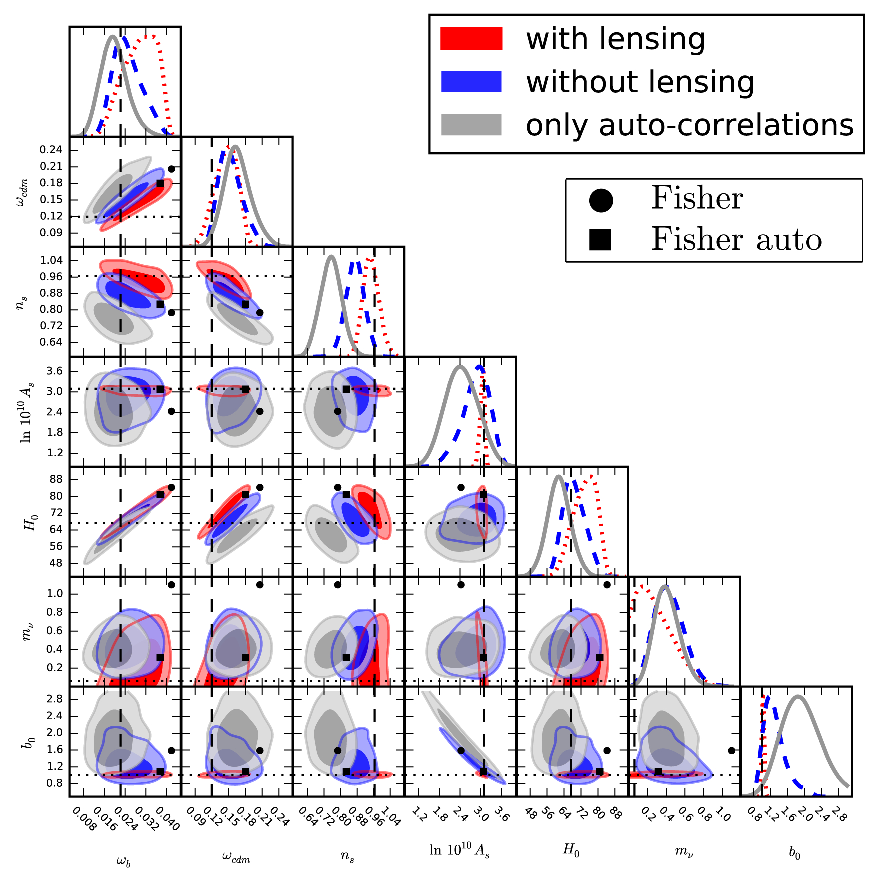
\includegraphics[width=\textwidth]{figures/chapter-mnu/triangle_figure_MCDM_bias_w_legend.pdf}
  \caption{Two- and 1-D posteriors for the cosmological parameters inferred from the full analysis including lensing (red dotted), an analysis neglecting lensing (blue dashed) and considering only auto-correlations (gray solid).
    The 68\% and 95\% confidence intervals are shown.
    Intersections between vertical and horizontal lines denote the fiducial cosmology.
   In this analysis no significant priors were imposed on the parameters.  Circles and squares represent the estimates for the best-fits from a Fisher matrix analysis when neglecting lensing, and for the only auto-correlations case, respectively.
  }
  \label{fig:mcmc}
\end{figure*}

%We have  fitted the generated $C_\ell^{ij}$ data in three different ways,  where lensing convergence is: i) consistently included, ii) neglected, iii) neglected and only redshift bin auto-correlations are taken into account. 

%The results are shown in Table~\ref{Table:1} and Figure~\ref{fig:mcmc}. Fig.~\ref{fig:mcmc} shows 2D contours and 1D probability distribution functions for the marginalized posteriors of the cosmological parameters obtained from these analyses. The red contours (dotted 1D distributions) show the full analysis. They should reproduce the fiducial model. In the analyses shown by the gray (1D solid) and blue (1D dashed) contours lensing is neglected. Furthermore, in the gray  contours only auto-correlations (i.e.\ $C_\ell(z,z)$) are considered, while the blue contours use both auto- and cross-correlations (i.e.\ $C_\ell(z,z')$ for all combinations of redshift bins).
%The auto-correlation case is closer to the standard $P(k)$ analysis which is usually performed in redshift bins, but caution should be taken in comparing the two analyses since binning in redshift has significantly different effects.

The analysis that consistently includes lensing convergence (red contours in Figure \ref{fig:mcmc}) should output the fiducial model. The corresponding constraints in Table \ref{Table:1} show that the best fitting parameters are indeed very close to the input fiducial parameters (see the amplitude of the shift of the best fit). The amplitude of the shifts of the mean of some parameters (i.e., $m_\nu$, $H_0$, $\omega_{cdm}$, $\omega_b$) reveal the limitations of our analysis. On the one hand, since the main impact of massive neutrinos occurs on small scales and we treat non-linear scales very conservatively, an improvement on the constraints of the neutrino absolute mass scale is expected in an analysis including, for instance, scales up to $\ell=2000$. On the other hand, the universe's expansion rate, the reduced baryon density parameter, and the cold dark matter density parameter are not well constrained due to degeneracies in these parameters (see Figure \ref{fig:mcmc}). These degeneracies come from the dominant contributions in the matter transfer function that are basically fixed by the ratio $\omega_b/\omega_{\mathrm{cdm}}$ and by the scale of the particle horizon at the radiation-matter equality epoch $z_{\mathrm{eq}}$ \cite{Eisenstein:1997ik}. The equality scale $k_{\rm eq}$ behaves like  
\begin{equation}
k_{\rm eq} \propto \frac{\omega_m}{H_0},
\end{equation}      
where we assume a fixed radiation content and measure $k_{\rm eq}$ in $h/ \Mpc$.  
%From the red contours in Fig.~\ref{fig:mcmc} it is evident that we cannot determine the baryon and cold dark matter densities very well with our configuration. The rather large redshift bins of our analysis with $\Delta z\gtrsim 0.3$ significantly smear out the baryon acoustic oscillations (BAO's), leaving only the dominant features in the power spectrum which are fixed by the equality scale, $k_{\rm eq} \propto \omega_m/H_0$ (at fixed radiation content and measured in $h/$Mpc) and the ratio $\omega_b/\omega_{\mathrm{cdm}}$. This  leads to a significant  degeneracy between $\omega_b$, $\omega_{\rm cdm}$ and $H_0$, only the slopes of the $(\omega_x,H_0)$ and the $(\omega_b, \omega_{\rm cdm})$  contours are well determined. The large uncertainties in these parameters, as well as the prior $m_\nu\geq 0$, push the posterior mean value away from the best fit (which is always very close to the input value). We did not add realization noise in our likelihood, since it is not relevant for the present study.
%Our aim here is not to derive optimal parameter constraints, but to demonstrate the importance of the lensing contribution in such an analysis. For this reason our approach is far from optimal but  conservative and simple, and even in this case we find that not including lensing leads to wrong results.
%Optimizing error contours by, e.g., introducing more non-linear scales in the analysis is expected to lead to even more biased results, given  that  the relevance of lensing increases at higher multipoles.

Gray contours in Figure \ref{fig:mcmc} show the analysis neglecting lensing, but including only red-shift bin auto-correlations. The effective $\Delta \chi^2$ for this case is greater than in the case consistently including lensing, thus suggesting that the model neglecting lensing has difficulties in fitting the mock data. The spectral index and the neutrino mass are significantly biased ($>2.5\sigma$) from the input fiducial parameters. Moreover, a degeneracy between the bias parameter $b_0$ and the amplitude of scalar fluctuations $A_s$ appears. This comes from the fact that the product $A_s b_0^2$ determines the overall amplitude of matter fluctuations and therefore its increase (decrease) signifies an enhancement (decrement) of power on all scales. The bias on $n_s$ and $m_\nu$ can be understood as follows. Since the magnification bias in $s(z)$ Eq. \eqref{Eq:magnification-bias} is relatively large (see Figure \ref{fig:bs}), the density-lensing correlation term
\begin{equation}
b(z)(5s(z)-2)\langle D \kappa \rangle,
\end{equation}   
contributes to the power with a positive (negative) sign for red-shift bins with $z>1$ ($z<1$). Because correlations of relatively small red-shifts bins probe mainly small scales, the decrement of power on small scales due to lensing convergence must be corrected in a model no including lensing. This correction can be achieved by lowering the spectral index -- since $P(k) \propto k^{n_s -1}$ -- and increasing the neutrino mass.

Finally, we focus our attention on the analysis that neglects lensing convergence, but includes all red-shift bin correlations (blue contours in Figure \ref{fig:mcmc}). Although bias on cosmological parameters appear to be smaller in this case -- as compared to the gray contours --, this improvement is not significant. Since the lensing term might actually dominate the radial power spectrum at large scales \cite{Bonvin:2011bg}, it is even more difficult for a model that neglects lensing and includes cross-correlations to fit the mock data. This is easily seen with the value of the effective $\Delta \chi^2$ in Table \ref{Table:1}. The $\Delta \chi^2$ increases from $\Delta \chi_{\rm auto}^2\simeq 180$ for the five auto-correlation bins to more than $\Delta \chi_{\rm a+c}^2\gtrsim2000$ when adding the 10 cross-correlation bins. If one naively gives each bin the same weight,  one would expect an increase by a factor 3. We however find an increase
$\Delta \chi_{\rm a+c}^2/\Delta \chi_{\rm auto}^2\gtrsim 11$.   

Models with additional parameters, but neglecting lensing convergence are likely to weaken the constraints -- introducing new degeneracies -- and produce even stronger biases on the cosmological parameters. Therefore, from the analyses presented above, we conclude that to go beyond the current state and derive accurate estimates of the absolute neutrino mass scale with galaxy surveys absolutely requires taking lensing convergence into account. Figure \ref{fig:cl}   shows number counts angular power spectra for analyses including and neglecting lensing computed at the corresponding best fit (see Table \ref{Table:1}). The thick red lines indicate the model including lensing and the thin blue lines show the model neglecting lensing (including all red-shift bin cross-correlations). For the spectra of the model consistently including lensing, we show 1-$\sigma$ error bars that were computed by assuming Gaussian spectra (see Eq.~(2.13) of \cite{Montanari:2015rga}). Correlations between the red-shift bins $(ij)=(11), ~(55)$ and $(15)$ are shown. One can see that when neglecting lensing, the spectrum for the cross-correlation between red-shift bins $1$ and $5$ lies outside the 1-$\sigma$ error bars around the fiducial spectrum including lensing. This clearly evidences that a  model neglecting lensing convergence cannot fit the mock data.

%If lensing is neglected in the analysis, several parameters
%show a significant bias with respect to the input parameters (given by the vertical dashed lines)  cf. also Table~\ref{Table:1}.
%First of all, there is a very strong degeneracy between the scalar amplitude $A_s$ and the bias $b_0$.  When including lensing which does not depend on $b_0$ this degeneracy is broken and both, $b_0$ and $A_s$ are determined accurately. Furthermore, lensing (together with the magnification bias for Euclid specifications) enhances clustering. Compensating this with a larger value of $b_0^2A_s$ leads to too much clustering on small scales, which, in turn, is compensated by reducing the spectral index by $(2-4)\sigma$ and by increasing the neutrino mass.   The preferred neutrino mass
%is around $0.4\, \mathrm{eV}$, which corresponds just about to the current limits from cosmology~\cite{Ade:2015xua}.
%From the degeneracy directions in the two-dimensional contours in Fig.~\ref{fig:mcmc}
%we can also read off that forcing $m_\nu \rightarrow m_\nu^{\rm (fid)} = 0.06\, \mathrm{eV}$ would lead to
%an even larger bias in the scalar spectral index.


%It is interesting that taking cross-correlations into account helps somewhat to reduce the bias on the parameters. The scalar spectral index best-fit in this case has a bias of $1.8\sigma$,  as compared to $3.8\sigma$ for auto-correlations only, and the neutrino mass is shifted by $2.2 \sigma$ compared to $2.5\sigma$,
%see Table~\ref{Table:1}. But this `improvement' is actually not real. It comes to a big extent from the fact that cross-correlations simply cannot be fitted without the lensing term as discussed below and shown in Fig.\ \ref{fig:cl}.  This is most manifest in the  total $\Delta \chi^2$ which increases from $\Delta \chi_{\rm auto}^2\simeq 180$ for the five auto-correlation bins to more than $\Delta \chi_{\rm a+c}^2\gtrsim2000$ when adding the 10 cross-correlation bins. Giving each bin naively the same weight we would expect an increase by a factor 3, instead we have
%$\Delta \chi_{\rm a+c}^2/\Delta \chi_{\rm auto}^2\gtrsim 11$.
%The increase in the size of the parameter contours for some parameters appears at first counter-intuitive as including more data improves our knowledge and therefore should reduce the errors.
%This simple logic, however, only applies if the data can actually be fitted by the model at hand or if the likelihoods are Gaussian. Otherwise, different data may prefer different model parameters and lead to an increase not only in the total $\Delta \chi^2$ but also in the size of the confidence contours.



\begin{figure}[tp]
  \centering
  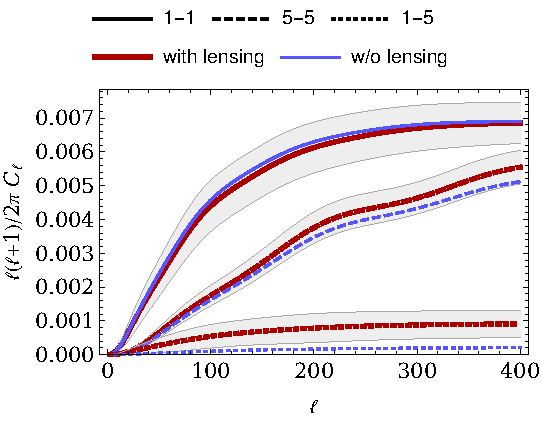
\includegraphics[width=\columnwidth]{figures/chapter-mnu/fid_shift.pdf}
  \caption{
    The thick red and the thin blue lines correspond to the spectra at the best-fit values estimated by consistently including lensing and by neglecting it, respectively.
    Gaussian error bars accounting for cosmic variance and shot-noise for the consistent analysis are shown as gray regions.
    The indices for the correlated redshift bins are shown in the legend.
    The model neglecting lensing cannot fit the data, especially due to redshift cross-correlations.
  }
  \label{fig:cl}
\end{figure}


\begin{table}[!t]
  \centering
  \begin{tabular}{c|cccc}
    Parameter & \multicolumn{2}{c}{Shift of best-fit } &\multicolumn{2}{c}{for MCMC} \\
    \hline
       $\omega_b$ & $1.2\sigma$ & ($0.9\sigma$) & $-0.1\sigma$ & ($-0.9\sigma$)\\
   $\omega_{cdm}$ & $1.7\sigma$ & ($1.1\sigma$)& $1.1\sigma$ &
($1.5\sigma$)\\
   $n_s$      & $-1.9\sigma$ & ($-1.3\sigma$) & $-1.8\sigma$ &
($-3.8\sigma$) \\
   $\ln10^{10}A_s$ & $-1.1\sigma$ & ($0.005\sigma$)& $-0.3\sigma$ &
($-0.8\sigma$)\\
   $H_0\left[\frac{\text{km}}{\text{s}\cdot\text{Mpc}}\right]$ &
$1.2\sigma$ & ($0.9\sigma$)& $-0.1\sigma$ & ($-1.5\sigma$)\\
   $m_{\nu}$\,[eV]  & $3.3\sigma$ & ($0.6\sigma$)  & $2.2\sigma$ &
($2.5\sigma$)\\
   $b_0$      & $1.7\sigma$ & ($0.1\sigma$)   & $0.7\sigma$ &
($1.4\sigma$)\\
  \end{tabular}

  \caption{
      Fisher matrix results for the shift in the best-fit values due to neglecting lensing, in units of standard deviations (see Figure \ref{fig:fisher}). The numbers in parenthesis refer the the case including only bin auto-correlations. For comparison we also give in columns 4 and 5 the corresponding values from the MCMC analysis presented in Table~\ref{Table:1} and Fig.~\ref{fig:mcmc}. While Fisher matrices give a good qualitative description of parameter degeneracies, estimates of the shifts in the best-fits seriously misestimate the magnitude and direction in parameter space.
 }
  \label{Table:Fisher}
\end{table}

\begin{figure*}[bthp]
  \centering
  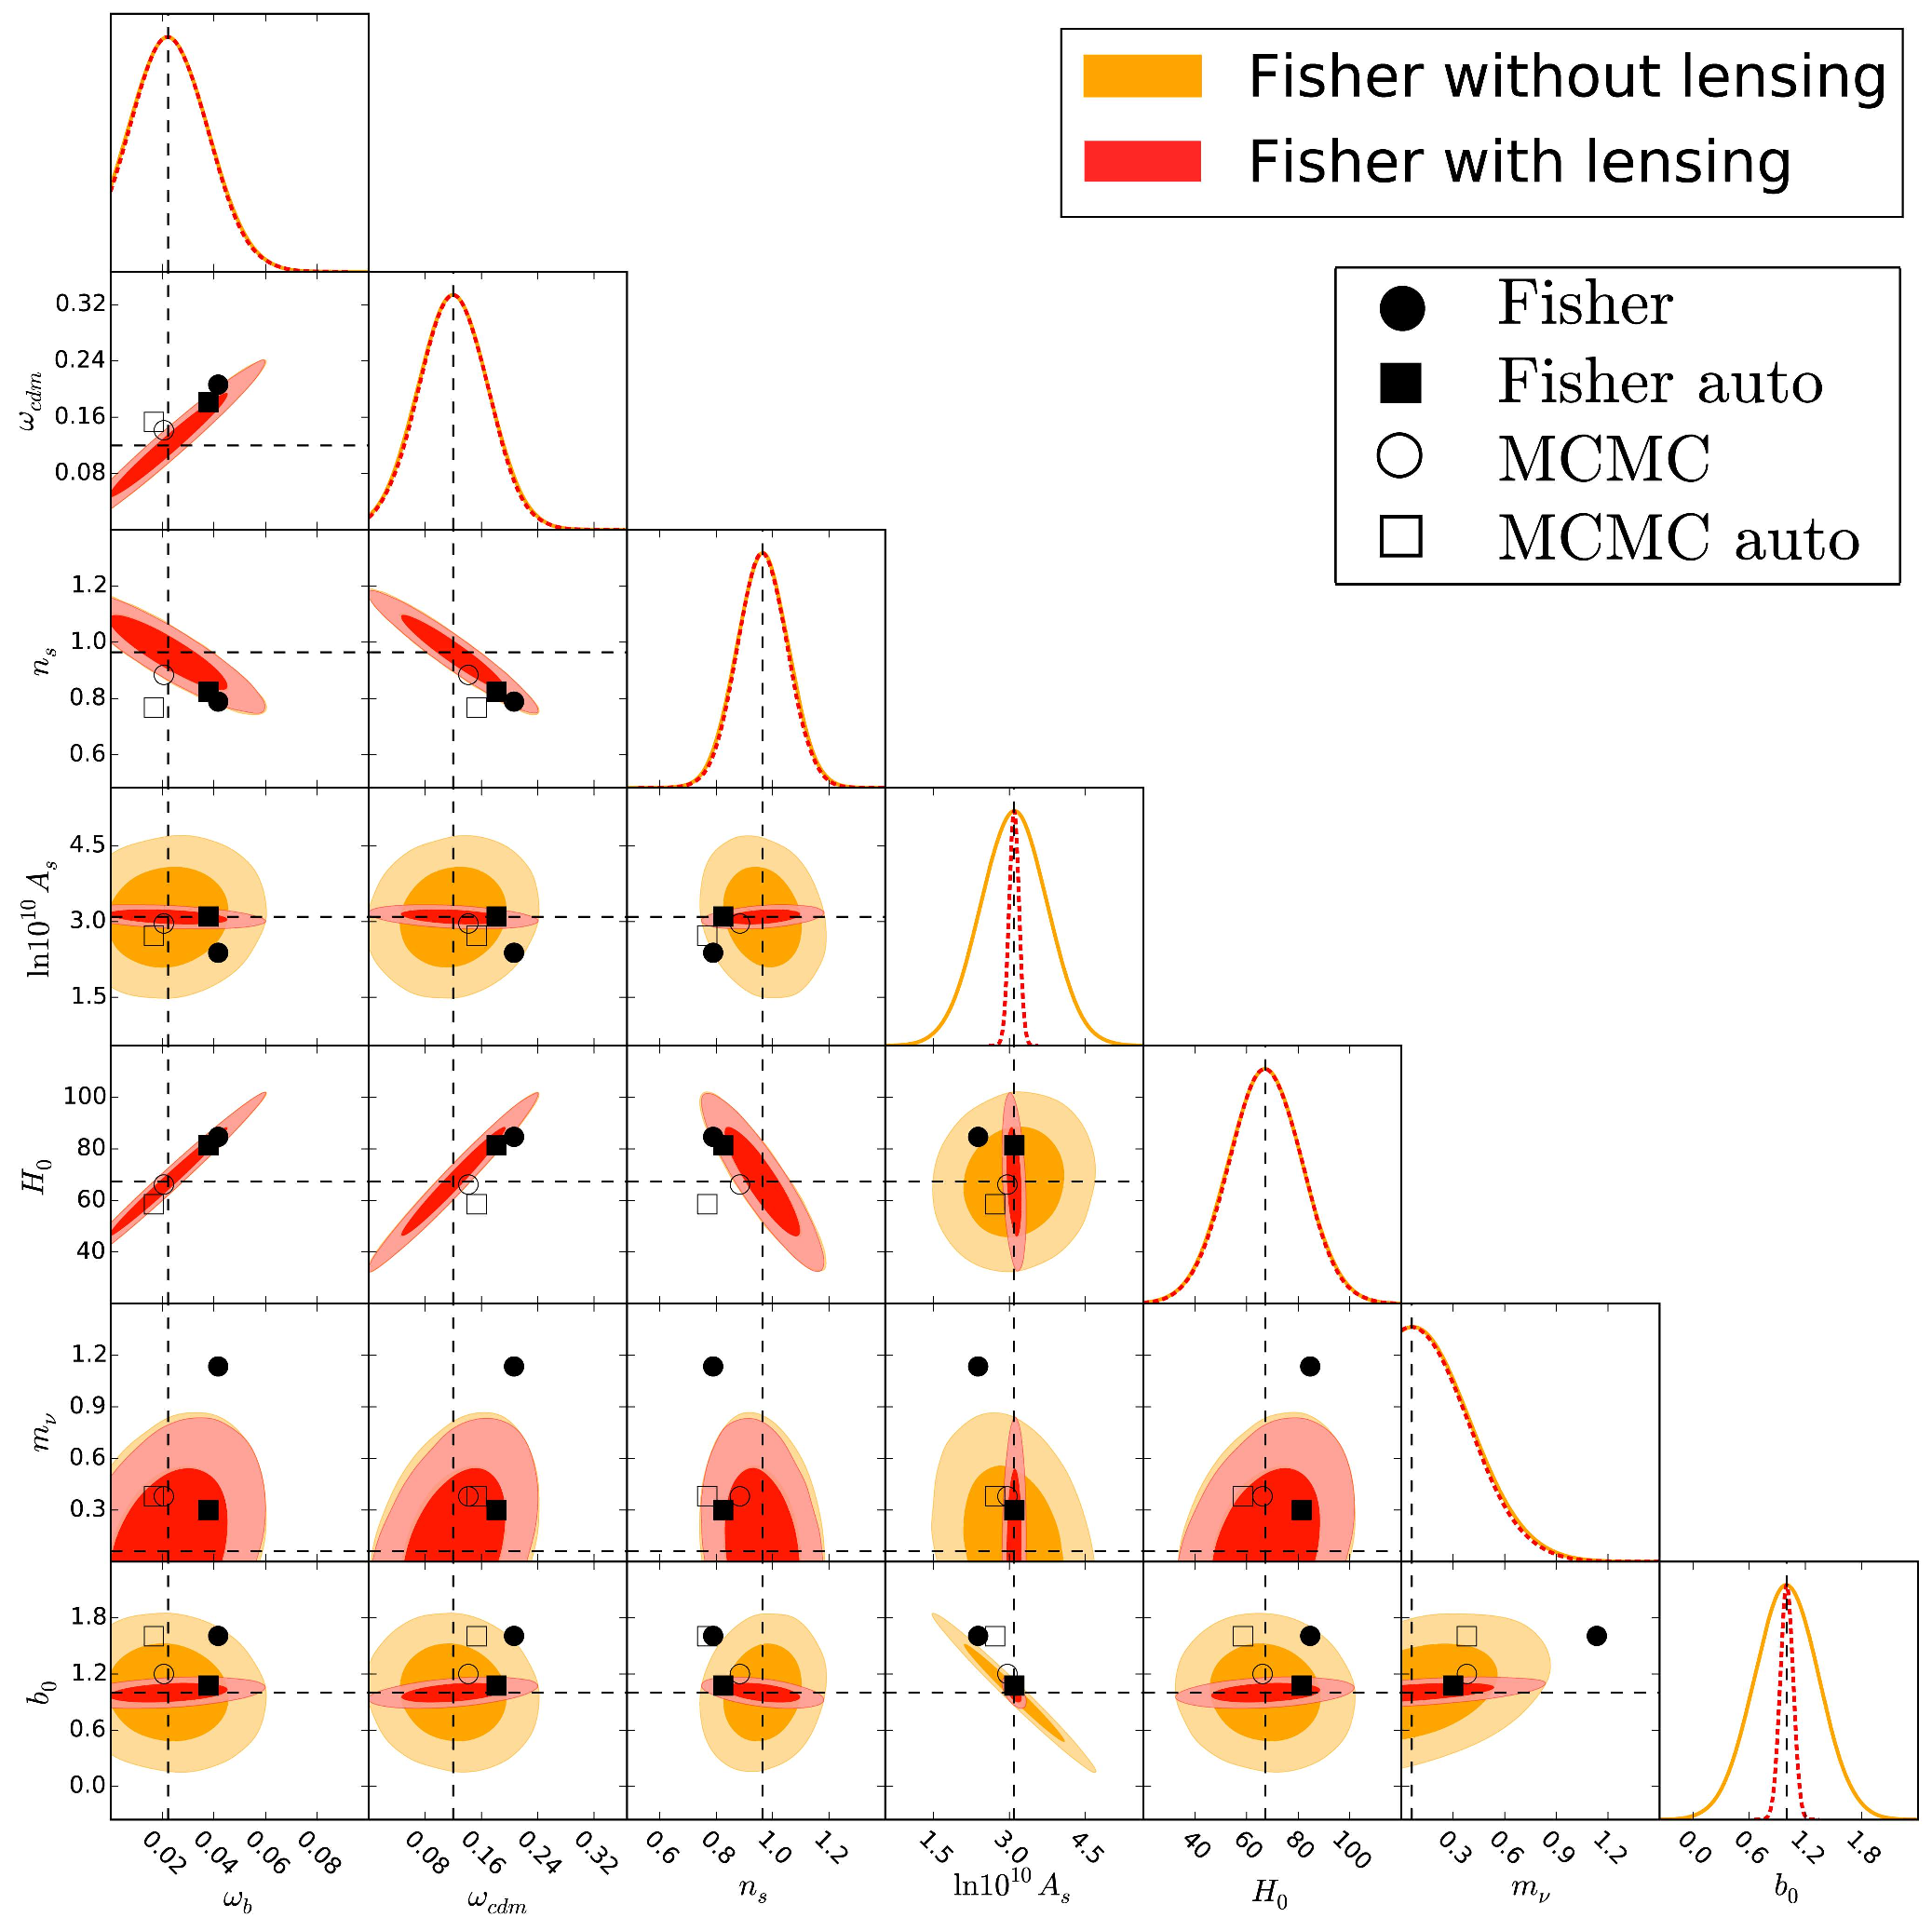
\includegraphics[width=\textwidth]{figures/chapter-mnu/triangle_figure_Fisher_bias.pdf}
  \caption{
      Two- and 1-D posteriors for the cosmological parameters inferred from the Fisher analysis excluding (orange solid) and including lensing (red dotted).
    We stress that, in the former case, to compute error ellipses within the Fisher formalism we forecast parameter constraints in a Universe where lensing is absent (see the text for more details).
    The 68\% and 95\% confidence intervals are shown.
    Intersections of dashed lines denote the fiducial cosmology.
The expected systematic shifts in the best-fit due to neglecting lensing in the theoretical modeling are shown, including all bin correlations (circles), and including only auto-correlations (squares).
For comparison, we also show the corresponding results from the MCMC analysis.
While the Fisher formalism is reliable for a qualitative understanding of parameter degeneracies, the systematic errors are seriously misestimated.
    See table \ref{Table:Fisher} for more details about statistical quantities.
}
  \label{fig:fisher}
\end{figure*}

\subsection{Fisher analysis without priors}\label{s:fisher}

An alternative, widely used approach to make forecasts is the Fisher matrix method \cite{Namikawa:2011yr,Duncan:2013haa,Camera:2014sba,Raccanelli:2015vla}. In this subsection, we compare how well a Fisher matrix technique performs as compared to the MCMC method of the precedent subsection. Since we have seen the biases on cosmological parameters might reach several standard deviations when neglecting lensing convergence in the analysis, we expect the Fisher matrix forecasts to be not very reliable (see Section \ref{chapter-mnu:methodology}). The basic expressions of the Fisher matrix formalism are explained in the Appendix \ref{appendix2-mnu}.
 
The figure \ref{fig:fisher} shows two- and 1-D posteriors for two Fisher analyses. Red contours indicate forecasts for an analysis consistently including lensing convergence, whereas yellow contours show results for an analysis where lensing is neglected (not only in the model, but also in the underlying universe). Red contours in both Figure \ref{fig:mcmc} and Figure \ref{fig:fisher} can therefore be directly compared. The shifts of the best fit parameters for analyses neglecting lensing are computed as explained in Appendix \ref{appendix2-mnu} and shown in Table \ref{Table:Fisher}. The standard deviations $\sigma$ in this Table refer to the model neglecting lensing which provides more conservative information about the importance of the systematic error. 
%We stress that in both cases, without and with lensing, Fisher matrices only forecast error contours around a universe described by the fiducial parameters and assume a Gaussian likelihood.
%  While the MCMC analysis allows us to fit the wrong or the correct model to the data, in the Fisher context this is not possible.
%  E.g., in the case without lensing we ask the outcome of fitting a model without lensing to a Universe without lensing.
%  Hence, while the red dotted contours `with lensing' can be compared between Figures \ref{fig:mcmc} and \ref{fig:fisher}, the other contours have no correspondence between the two figures.

Comparing Figures \ref{fig:mcmc} and \ref{fig:fisher}, we can see that the Fisher matrix analysis provides a good qualitative description of degeneracy between different parameter constraints. Although the 68\% confidence intervals are in disagreement with MCMC results by a factor 2-3, the shape and inclination of the ellipses very roughly follow the MCMC contours. On the other hand, the Fisher matrix analysis badly fails in determining the magnitude and direction of the best-fit shift in parameter space. Indeed, the first-order formalism that we use to estimate the shift in the best-fitting parameters due to a systematic error -- neglecting lensing convergence -- is valid as long as the shift is small compared to the errors, and it also assumes that the systematic error does not affect the ellipse contours \cite{Kitching:2008eq}. The results from the MCMC approach in the previous subsection and the contours depicted in Figure \ref{fig:fisher} clearly show that these assumptions are not fulfilled in the present case.

\subsection{MCMC with Planck Gaussian prior}

As discussed above, degeneracies in parameter space limit the constraints from measurements of the galaxy power spectrum. This difficulty is usually tackled by applying a variety of priors or constraints on parameters, and combining the galaxy clustering data with other cosmological measures, such as CMB experiments \cite{Tegmark:2003ud}. We therefore
repeat our MCMC analysis using Planck priors for all the cosmological parameters except the bias $b_0$, which is not measured in {\it Planck}, and the neutrino mass. The latter is our most interesting parameter and we want to test how strongly it is biased in an analysis which neglects lensing.

{\it Planck} chains are publicly available through the \textit{Planck Legacy Archive}. In this paper we use the chain for the extended model with a free neutrino mass based on the {\it Planck} TT, TE, EE + lowP likelihoods (Equation [54c] in \cite{Ade:2015xua}). We compute the covariance matrix $\mathbf{C}$ for the cosmological parameters $\vec{x}=(\omega_b,\omega_{\mathrm{cdm}},n_s,A_s,H_0)$ and assume a Gaussian distribution for the prior. The $\chi^2$ relative to the fiducial model including the Planck prior is then the $\Delta \chi^2$ in Eq. \eqref{Eq:relative-chi2} plus
\begin{equation}
\Delta \chi^2_{\mathrm{prior}} = \sum_{i,j} (x_i - x^{\mathrm{fid}}_i) C^{-1}_{ij} (x_j - x^{\mathrm{fid}}_j),
\label{Eq:chi2-prior}
\end{equation}
where $\vec{x}^{\mathrm{fid}}$ denotes parameters of the fiducial model and $\mathbf{C^{-1}}$ is the inverse of the covariance matrix. In this way we marginalize the Planck prior over the neutrino mass and the optical depth, $\tau$, which are parameters that we want to leave free since we want to determine the first and our survey is not sensitive to the second. The results are shown in Table~\ref{Table:2} and Fig.~\ref{fig:mcmc-cmb-prior}.

Red contours in Figure \ref{fig:mcmc-cmb-prior} indicate the full analysis including lensing convergence. Adding CMB information clearly helps to remove degeneracies and cosmological parameters are now better determined than for the case with wide, flat priors. Blue and gray contours show analyses neglecting lensing convergence. While the spectral index $n_s$ shows now a smaller relative shift, the neutrino masses and galaxy bias actually acquire larger shifts. Since the model neglecting lensing must correct the number counts angular power spectrum on small scales by increasing neutrino mass and lowering spectral index, the Hubble parameter $H_0$ is pulled away from the fiducial value by over $4\sigma$ in spite of the Planck prior. Hence, while the details of the analysis are important in determining the actual size of error bars and degeneracies in parameter space, a large bias $2\sigma$--$9\sigma$ in the neutrino masses is a feature that persists in all the analyses here performed. Lensing convergence must be included when analysing data from future galaxy surveys, otherwise constraints on the neutrino mass will be in a high degree biased.  


\begin{table}[!t]
  \centering
  \begin{tabular}{@{}cccccc}
    \hline
    \multicolumn{6}{c}{i) Consistently including lensing: $\Delta \chi^2 = 0$} \\
    \hline
    Parameter & Mean & best fit & $\sigma$ &\hspace{-0.52cm} shift: mean & best-fit \\
    \hline
    $\omega_b$ & $0.02223$ & $0.02226 $ &$0.00013 $ &  \quad$0.2\sigma$ & $ <0.1\sigma$ \\
    $\omega_{cdm}$ & $0.1200 $ & $0.1196 $ & \quad$0.0011 $ &  \quad$0.2\sigma$ & $0.2\sigma$ \\
    $n_s$      & $0.9642 $ & $0.9651 $ & $0.0041 $ &  \quad$0.1\sigma$ & $ 0.1\sigma$ \\
    $\ln10^{10}A_s$ & $3.092 $ & $3.098$ & $0.026 $ &  \quad$0.1\sigma$ & $ 0.2\sigma$ \\
    $H_0\left[\frac{\text{km}}{\text{s}\cdot\text{Mpc}}\right]$      & $67.08$ & $67.25$ & $0.70$ &  \quad$0.3\sigma$ & $ <0.1\sigma$ \\
    $m_{\nu}$\,[eV]  & $0.08$ & $0.04$ & $0.05$ & \quad $ 0.4\sigma$ & $ 0.4\sigma$ \\
    $b_0$ & $1.005$ & $0.994$ & $0.018$ & $0.3\sigma$ & $0.3\sigma$ \\
  \end{tabular}
  \begin{tabular}{@{}cccccc}
    \hline
    \multicolumn{6}{c}{ii) Neglecting lensing: $\Delta \chi^2 = 2082$} \\
    \hline
    Parameter & Mean & best fit & $\sigma$ & \hspace{-0.52cm} shift: mean & best-fit \\
    \hline
    $\omega_b$ & $0.02220$ & $0.02219 $ & $0.00017 $ &  \quad$0.3\sigma$ & $0.4\sigma$ \\
    $\omega_{cdm}$ & $0.1215$ & $0.1214$ & $0.0014$ &  \quad$1.2\sigma$ & $1.1\sigma$ \\
    $n_s$      & $0.9643$ & $0.9640$ & $0.0049$ &  \quad$<0.1\sigma$ & $0.1\sigma$ \\
    $\ln10^{10}A_s$ & $ 3.085 $ & $3.090 $ & $ 0.034 $ &  \quad$0.3\sigma$ & $0.1\sigma$ \\
    $H_0\left[\frac{\text{km}}{\text{s}\cdot\text{Mpc}}\right]$      & $65.66$ & $65.64$ & $0.87$ &  \quad$1.8\sigma$ & $1.9\sigma$ \\
    $m_{\nu}$\,[eV]  & $0.35$ & $0.34$ & $0.06$ &  \quad$4.8\sigma$ & $4.7\sigma$ \\
    $b_0$ & $1.072$ & $1.070$ & $0.022$ & $3.3\sigma$ & $3.3\sigma$\\
  \end{tabular}
  \begin{tabular}{@{}cccccc}
    \hline
    \multicolumn{6}{c}{\parbox[t]{4.4cm}{iii) Neglecting lensing: \\ \hspace*{0.9cm} (only auto-correlations)} $\Delta \chi^2 = 230$} \\
    \hline
    Parameter & Mean & best fit & $\sigma$ & \hspace{-0.52cm} shift: mean & best-fit\\
    \hline
    $\omega_b$ & $0.02185 $ & $0.02181 $ & $0.00014 $ &  \quad$2.8\sigma$ & $3\sigma$ \\
    $\omega_{cdm}$ & $0.1240 $ & $0.1240 $ & $0.0013 $ &  \quad$3.4\sigma$ & $3.3\sigma$ \\
    $n_s$      & $0.9529 $ & $0.9536 $ & $0.0044 $ &  \quad$2.7\sigma$ & $2.5\sigma$ \\
    $\ln10^{10}A_s$ & $3.079 $ & $3.081 $ & $0.033 $ &  \quad$0.5 \sigma$ & $0.4\sigma$ \\
    $H_0\left[\frac{\text{km}}{\text{s}\cdot\text{Mpc}}\right]$      & $62.72 $ & $62.71$ & $1.01$ &  \quad$4.5 \sigma$ & $4.5\sigma$ \\
    $m_{\nu}$\,[eV]  & $0.50$ & $0.52$ & $0.05$ &  \quad$8.6\sigma$ & $8.8\sigma$ \\
    $b_0$ & $1.127$ & $1.127$ & $0.022$ & $5.7\sigma$ & $5.7\sigma$ \\
  \end{tabular}
 \caption{MCMC results with Planck priors. We show the mean and best fit values, the standard deviation and the amplitude of the shift of the mean and best-fit w.r.t. the fiducial value in units of the standard deviation, $\sigma$, of the corresponding analysis. The large value of $\Delta \chi^2$ for case ii) shows that cross-correlations cannot be fitted if lensing is neglected.
  }
  \label{Table:2}
\end{table}


\begin{figure}[bthp]
  \centering
  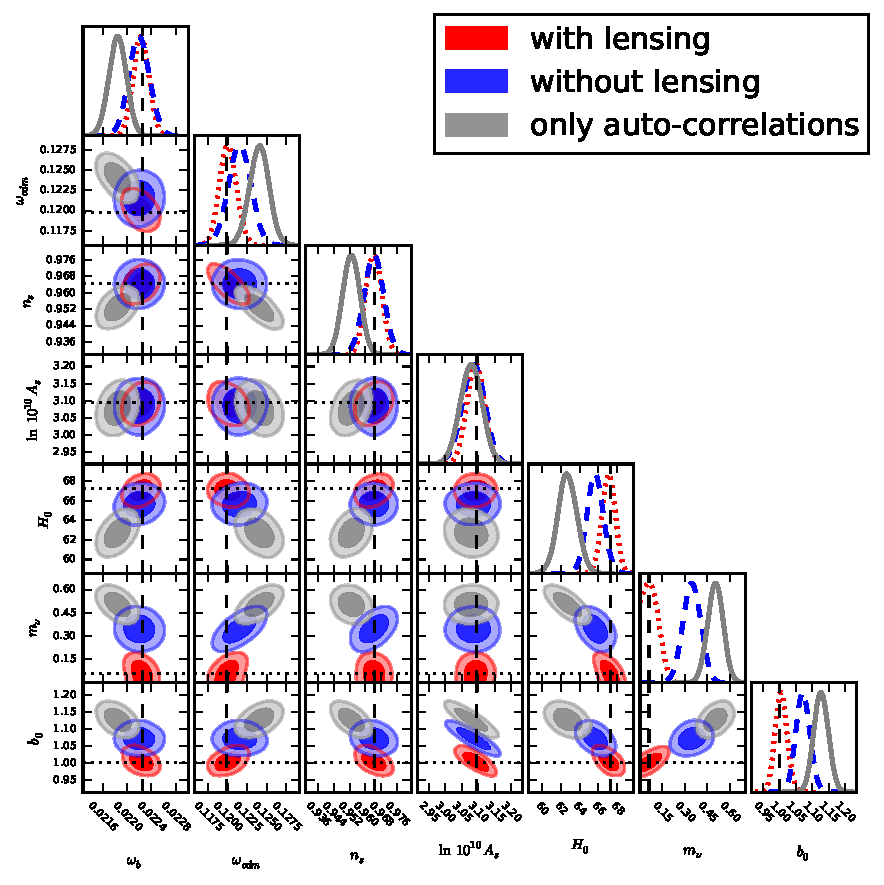
\includegraphics[width=\textwidth]{figures/chapter-mnu/triangle_figure_MCDM_bias_cmb_prior.pdf}
  \caption{Two- and 1-D posteriors for the cosmological parameters inferred using Planck priors. We show the full analysis including lensing (red dotted), an analysis neglecting lensing (blue dashed) and considering only auto-correlations (gray solid).
    The 68\% and 95\% confidence intervals are shown.
    Intersections between vertical and horizontal lines denote the fiducial cosmology.
   See Table \ref{Table:2} for numerical values of the statistical quantities.
  }
  \label{fig:mcmc-cmb-prior}
\end{figure}

\subsection{Significance of the lensing detection}

We can quantify the strength with which we detect the lensing signal in our setup with the help of Bayesian model probabilities, comparing the case with lensing to the case without lensing. To do this, we introduce formally an extended model $\MM_L$ with an additional `lensing amplitude' parameter $A_L$ that multiplies the lensing contribution in the model. For the `with lensing' model $\MM_1$ we then set $A_L = 1$, while the `without lensing' case $\MM_0$ corresponds to $A_L=0$. In this way the two models are nested within the extended model and we can use the Savage-Dickey density ratio (SDDR) method to derive model probabilities (see e.g.\ \cite{Trotta:2005ar} for an explanation of the SDDR, and section 3 of \cite{Dirian:2016puz} for a more detailed description of the same reasoning as the one used here): with the SDDR, the Bayes factor $B$ between the case with fixed $A_L$ and the general case is given by the posterior for $A_L$ (marginalised over all other parameters) of the general model divided by prior, both taken at the nested point,
\begin{equation}
B_x \equiv \frac{P(D|\MM_x)}{P(D|\MM_L)} = \frac{P(A_L=x|D,\MM_L)}{P(A_L=x|\MM_L)} \, ,
\end{equation}
where $P$ denote probabilities, $D$ the data and $x$ is either 0 or 1.
%$\theta$ the other parameters in the model.
The Bayes factor between two models with given fixed values for $A_L$ is then simply the ratio of the Bayes factors relative to the extend model, 
\begin{equation}
B_{xy} \equiv \frac{P(D|\MM_x)}{P(D|\MM_y)} \nonumber
\end{equation}
\begin{eqnarray}
&=& \frac{P(D|\MM_x)}{P(D|\MM_L)} \frac{P(D|\MM_L)}{P(D|\MM_y)} = \frac{B_x}{B_y} \nonumber \\
 &=& \frac{P(A_L=x|D,\MM_L)}{P(A_L=y|D,\MM_L)} \, ,
\end{eqnarray}
where the last equality holds if $P(A_L=x|\MM_L)=P(A_L=y|\MM_L)$, e.g.\ for an uniform prior in $A_L$, which is what we will use. We see that the only information needed to determine $B_{xy}$ is the relative value of the posterior at $A_L=x$ and at $A_L=y$, and this is approximately given by the $\chi^2$ difference between these cases. As by construction $A_L=1$ (the case where we include lensing consistently) has $\Delta\chi^2=0$, we find simply that $\ln B_{01} \approx -\Delta\chi^2_{\mathrm{no~lensing}}/2$. We find thus that $\ln B_{01} \approx -1000$ when using auto- and cross-correlations, and $\ln B_{01} \approx -90$ to $-115$ when only taking into account autocorrelations. Both Bayes factors are way out on the often-used Jeffreys' scale \cite{Jeffreys:1939xee} where anything larger than 5 is considered as strong. In other words, lensing is detected in both cases with an overwhelming evidence.

We can also translate the $\Delta\chi^2$ value into an order-of-magnitude estimate of `the number of sigmas' with which we detect the lensing signal in our setup. Assuming a Gaussian probability distribution function for $A_L$ so that $\Delta\chi^2 \approx (A_L-1)^2/\sigma[A_L]^2$, we find that $\sigma[A_L]$ needs to be 0.022 in order to explain the observed $\Delta\chi^2$ values of 2064 and 2082. This implies that the lensing is measured roughly at the $45\sigma$  level. Lensing is clearly a strong signal in the photo-$z$ type survey that we have considered here. As also discussed above, most of the lensing signal is contained in the off-diagonal spectra. The $\Delta\chi^2$ values of 180 and 230 when only looking at the auto-correlations correspond to about $13\sigma$ to $15\sigma$, roughly comparable to the strength of the lensing detection in the {\it Planck} temperature power spectrum \cite{Ade:2015xua}.
%While it would be better for an accurate determination of the detection strength to include $A_L$ explicitly as a parameter in the MCMC, our discussion here provides at least an estimate of the strength of the signal.


This also confirms the result of~\cite{Montanari:2015rga}, which found that the lensing amplitude $A_L$ can be determined to an accuracy of the order of (1-2)\%  with a Euclid like photometric survey, with the constraints coming especially from the off-diagonal (inter-bin) correlations.


\section{Conclusions}
\label{chapter-mnu:conclusions}

Future galaxy surveys will probe scales comparable to the horizon. The come of all this new data will make necessary very careful analyses and appropriate modelling of the statistical properties of the matter density field. In this chapter we have investigated the impact of lensing convergence on constraints of cosmological parameters. We have utilised both MCMC and Fisher matrix approaches to study the importance of including lensing convergence when analysing galaxy clustering data. Although the Fisher matrix formalism provides qualitative information about degeneracies in the parameter space, it badly fails in determining quantitative estimations of shifts in the best fitting parameters. When performing the analysis with a MCMC approach we have found that biases of best fitting cosmological parameters might reach several standard deviations when lensing convergence is neglected in the analysis. Since the Fisher matrix technique is reliable only for shifts relatively small, this explains why Fisher matrix results wrongly estimate the bias on cosmological parameters: for shifts bigger than $2\sigma$ the linear approximation in the Fisher formalism breaks down. A MCMC method is therefore suitable as we have shown.

We have seen that analysis neglecting lensing convergence lead to biased cosmological constraints. The spectral index $n_s$ and the neutrino mass $m_\nu$ are particularly affected. When neglecting lensing a degeneracy between the amplitude of scalar fluctuations $A_s$ and the galaxy bias parameter $b_0$ appears. One understands this by noting that the product $b_0^2 A_s$ determines the amplitude of the matter power spectrum, so $b_0^2 A_s$ increases in analysis neglecting lensing to enhance power on all scales. Since the density-lensing contribution to the number counts angular power spectrum can become negative for small red-shift bins, therefore decreasing power on small scales, its effect can be mimic by changes on $n_s$ and $m_\nu$: decreasing the spectral index and increasing the neutrino mass one obtains a damped matter power spectrum on small scales.

Finally, we conclude by noting that the specific shifts on the best fitting cosmological parameters depend on the details of the survey. Although in this project we have used specifications for an Euclid-like survey, the important point is that a consistent analysis of galaxy clustering data must take into account the magnification bias defined by      
%In this paper we have shown that neglecting  lensing convergence leads to large shifts in the best fit values of cosmological parameters for the data sets
%available from future surveys. As in the CMB, where the lensing of the power spectra is detected at over $10\sigma$ \cite{Ade:2015xua},
%it will become mandatory to include lensing also in the analysis of galaxy surveys.

%In the case studied here we have seen mainly an increase in the neutrino mass $m_\nu$ and a decrease in the spectral index $n_s$ when neglecting lensing. Also the product $A_sb_0^2$ which determines the amplitude of fluctuations increases. This comes from the fact that the magnification bias for the Euclid specifications is relatively large~\cite{Montanari:2015rga} (see also Appendix~\ref{apa}), so that the  density-lensing correlation in bins with $z>1$ contributes with a positive sign. At smaller redshifts which mainly measure correlations on smaller scales this has to be corrected since there the total lensing term $\propto (5s-2)\kappa$ contributes negatively. This can be achieved by lowering $n_s$ and increasing the neutrino mass.

%We note that
%the specific shifts which we have obtained in our analysis depend  on the details of the survey. The main, generic result is that in order to estimate cosmological parameters reliably with future galaxy surveys, we have to correctly include lensing with the measured magnification bias function, $s(z)$, defined by
\begin{equation}
s(z)  \equiv \frac{\partial\log_{10} N(z,m<m_*)}{\partial m_*}\,,
\end{equation}
where $m_{\mathrm{lim}}$ is the limiting magnitude of the survey and $N(z,m)$ is the galaxy luminosity function of the survey at redshift $z$. Our results show that a correct modelling of number counts might lead to detection of lensing with high significance as in the case of CMB. The fact that deep galaxy surveys are so sensitive to lensing, however, is not only a curse but also a blessing. It means that these surveys will allow us to determine a map of the lensing potential at different redshifts, i.e.\ perform `lensing tomography' with galaxy clustering. This will be a very interesting alternative to lensing tomography with shear measurements proposed, e.g.\
in~\cite{Heavens:2003jx}. Both techniques are challenging but they have different systematic errors and allow valuable cross-checks. So clearly both paths should be pursued.
